\documentclass[11pt]{article}

\usepackage{times}
\usepackage{epsf}
\usepackage{epsfig}
\usepackage{amsmath, alltt, amssymb, xspace}
\usepackage{wrapfig}
\usepackage{fancyhdr}
\usepackage{url}
\usepackage{verbatim}
\usepackage{fancyvrb}

\usepackage{subfigure}
\usepackage{cite}
%\usepackage{cases}
%\usepackage{ltexpprt}
%\usepackage{verbatim}

%\topmargin      -0.70in  % distance to headers
%\headheight     0.2in   % height of header box
%\headsep        0.4in   % distance to top line
%\footskip       0.3in   % distance from bottom line

% Horizontal alignment
\topmargin      -0.50in  % distance to headers
\oddsidemargin  0.0in
\evensidemargin 0.0in
\textwidth      6.5in
\textheight     8.9in 


%\centerfigcaptionstrue

%\def\baselinestretch{0.95}


\newcommand\discuss[1]{\{\textbf{Discuss:} \textit{#1}\}}
%\newcommand\todo[1]{\vspace{0.1in}\{\textbf{Todo:} \textit{#1}\}\vspace{0.1in}}
\newtheorem{problem}{Problem}[section]
%\newtheorem{theorem}{Theorem}
%\newtheorem{fact}{Fact}
\newtheorem{define}{Definition}[section]
%\newtheorem{analysis}{Analysis}
\newcommand\vspacenoindent{\vspace{0.1in} \noindent}

%\newenvironment{proof}{\noindent {\bf Proof}.}{\hspace*{\fill}~\mbox{\rule[0pt]{1.3ex}{1.3ex}}}
%\newcommand\todo[1]{\vspace{0.1in}\{\textbf{Todo:} \textit{#1}\}\vspace{0.1in}}

%\newcommand\reducespace{\vspace{-0.1in}}
% reduce the space between lines
%\def\baselinestretch{0.95}

\newcommand{\fixmefn}[1]{ \footnote{\sf\ \ \fbox{FIXME} #1} }
\newcommand{\todo}[1]{
\vspace{0.1in}
\fbox{\parbox{6in}{TODO: #1}}
\vspace{0.1in}
}

\newcommand{\mybox}[1]{
\vspace{0.2in}
\noindent
\fbox{\parbox{6.5in}{#1}}
\vspace{0.1in}
}


\newcounter{question}
\setcounter{question}{1}

\newcommand{\myquestion} {{\vspace{0.1in} \noindent \bf Question \arabic{question}:} \addtocounter{question}{1} \,}

\newcommand{\myproblem} {{\noindent \bf Problem \arabic{question}:} \addtocounter{question}{1} \,}


\newcommand{\copyrightnoticeA}[1]{
\vspace{0.1in}
\fbox{\parbox{6in}{\small Copyright \copyright\ 2006 - 2014\ \ Wenliang Du, Syracuse University.\\ 
      The development of this document is partially funded by 
      the National Science Foundation's Course, Curriculum, and Laboratory 
      Improvement (CCLI) program under Award No. 0618680 and 0231122. 
      Permission is granted to copy, distribute and/or modify this document
      under the terms of the GNU Free Documentation License, Version 1.2
      or any later version published by the Free Software Foundation.
      A copy of the license can be found at http://www.gnu.org/licenses/fdl.html.}}
\vspace{0.1in}
}


\newcommand{\copyrightnotice}[1]{
\vspace{0.1in}
\fbox{\parbox{6in}{\small Copyright \copyright\ 2006 - 2014\ \ Wenliang Du, Syracuse University.\\
      The development of this document is/was funded by three grants from
      the US National Science Foundation: Awards No. 0231122 and 0618680 from
      TUES/CCLI and  Award No. 1017771 from Trustworthy Computing.
      This lab was imported into the Labtainer framework by the Naval Postgraduate 
      School, Center for Cybersecurity and Cyber Operations under National Science 
      Foundation Award No. 1438893.
      Permission is granted to copy, distribute and/or modify this document
      under the terms of the GNU Free Documentation License, Version 1.2
      or any later version published by the Free Software Foundation.
      A copy of the license can be found at http://www.gnu.org/licenses/fdl.html.}}
\vspace{0.1in}
}

\newcommand{\copyrightnoticeB}[1]{
\vspace{0.1in}
\fbox{\parbox{6in}{\small Copyright \copyright\ 2006 - 2014\ \ Wenliang Du, Syracuse University.\\
      The development of this document is/was funded by the following grants from
      the US National Science Foundation: No. 0231122, 0618680, and 1303306.
      Permission is granted to copy, distribute and/or modify this document
      under the terms of the GNU Free Documentation License, Version 1.2
      or any later version published by the Free Software Foundation.
      A copy of the license can be found at http://www.gnu.org/licenses/fdl.html.}}
\vspace{0.1in}
}


\newcommand{\nocopyrightnotice}[1]{
\vspace{0.1in}
\fbox{\parbox{6in}{\small  
      The development of this document is funded by 
      the National Science Foundation's Course, Curriculum, and Laboratory 
      Improvement (CCLI) program under Award No. 0618680 and 0231122. 
      Permission is granted to copy, distribute and/or modify this document.
      }}
\vspace{0.1in}
}

\newcommand{\idea}[1]{
\vspace{0.1in}
{\sf IDEA:\ \ \fbox{\parbox{5in}{#1}}}
\vspace{0.1in}
}

\newcommand{\questionblock}[1]{
\vspace{0.1in}
\fbox{\parbox{6in}{#1}}
\vspace{0.1in}
}


\newcommand{\minix}{{\tt Minix}\xspace}
\newcommand{\unix}{{\tt Unix}\xspace}
\newcommand{\linux}{{\tt Linux}\xspace}
\newcommand{\ubuntu}{{\tt Ubuntu}\xspace}
\newcommand{\selinux}{{\tt SELinux}\xspace}
\newcommand{\freebsd}{{\tt FreeBSD}\xspace}
\newcommand{\solaris}{{\tt Solaris}\xspace}
\newcommand{\windowsnt}{{\tt Windows NT}\xspace}
\newcommand{\setuid}{{\tt Set-UID}\xspace}
%\newcommand{\smx}{{\tt Smx}\xspace}
\newcommand{\smx}{{\tt Minix}\xspace}
\newcommand{\relay}{{\tt relay}\xspace}
\newcommand{\isys}{{\tt iSYS}\xspace}
\newcommand{\ilan}{{\tt iLAN}\xspace}
\newcommand{\iSYS}{{\tt iSYS}\xspace}
\newcommand{\iLAN}{{\tt iLAN}\xspace}
\newcommand{\iLANs}{{\tt iLAN}s\xspace}
\newcommand{\bochs}{{\tt Bochs}\xspace}

\newcommand\FF{{\mathcal{F}}}

\newcommand{\argmax}[1]{
\begin{minipage}[t]{1.25cm}\parskip-1ex\begin{center}
argmax
#1
\end{center}\end{minipage}
\;
}

\newcommand{\bm}{\boldmath}
\newcommand  {\bx}    {\mbox{\boldmath $x$}}
\newcommand  {\by}    {\mbox{\boldmath $y$}}
\newcommand  {\br}    {\mbox{\boldmath $r$}}


%\pagestyle{fancyplain}
%\lhead[\thepage]{\thesection}      % Note the different brackets!
%\rhead[\thesection]{SEED Laboratories}
%\lfoot[\fancyplain{}{}]{Syracuse University} 
%\cfoot[\fancyplain{}{}]{\thepage} 

\newcommand{\tstamp}{\today}   
%\lhead[\fancyplain{}{\thepage}]         {\fancyplain{}{\rightmark}}
%\chead[\fancyplain{}{}]                 {\fancyplain{}{}}
%\rhead[\fancyplain{}{\rightmark}]       {\fancyplain{}{\thepage}}
%\lfoot[\fancyplain{}{}]                 {\fancyplain{\tstamp}{\tstamp}}
%\cfoot[\fancyplain{\thepage}{}]         {\fancyplain{\thepage}{}}
%\rfoot[\fancyplain{\tstamp} {\tstamp}]  {\fancyplain{}{}}

\pagestyle{fancy}
%\lhead{\bfseries Computer Security Course Project}
\lhead{\bfseries SEED Labs}
\chead{}
\rhead{\small \thepage}
\lfoot{}
\cfoot{}
\rfoot{}

\usepackage{listings}
\usepackage{color}

\definecolor{dkgreen}{rgb}{0,0.6,0}
\definecolor{gray}{rgb}{0.5,0.5,0.5}
\definecolor{mauve}{rgb}{0.58,0,0.82}

\lstset{frame=tb,
  language=C,
  aboveskip=3mm,
  belowskip=3mm,
  showstringspaces=false,
  columns=flexible,
  basicstyle={\small\ttfamily},
  numbers=none,
  numberstyle=\tiny\color{gray},
  keywordstyle=\color{blue},
  commentstyle=\color{dkgreen},
  stringstyle=\color{mauve},
  breaklines=true,
  breakatwhitespace=true,
  tabsize=3
}



\begin{document}

\begin{center}
{\LARGE Routing Basics}
\vspace{0.1in}\\
\end{center}

\section{Overview}
This exercise explores basic network routing concepts 
in a Linux environment.  These include use of the \texttt{route}
command to modify Linux routing tables, defining a DNS server in the /etc/resolv.conf file,
and an example of using Linux \textit{iptables} to implement Network Address Translation (NAT). 

Strictly speaking, this lab explores \textit{packet forwarding},
and not true network routing, which typically involves the use of
routing tables that name other network routers.  See the
\textit{bird-bgp} and \textit{bird-ospf} labs for examples of 
network routing.

This exercise, (and manual), is not intended to replace instruction
or independent reading on the topic of network packet forwarding and
routing in Linux systems. The exercise is intended to provide
students with an environment with which they can experiment
with the mechanics of forwarding network traffic to different network
interfaces based on Linux routing tables.  The student is only required
to view a simple example of using \textit{iptables} for NAT
in this lab.  See the {\tt iptables2} and the {\tt dmz} labs for a broader
look at iptables.

\section{Lab Environment}
This lab runs in the Labtainer framework,
available at http://nps.edu/web/c3o/labtainers.
That site includes links to a pre-built virtual machine
that has Labtainers installed, however Labtainers can
be run on any Linux host that supports Docker containers.

From your labtainer-student directory start the lab using:
\begin{verbatim}
    labtainer routing-basics
\end{verbatim}
\noindent A link to this lab manual will be displayed.  

\section{Network Configuration}
This lab includes a set of networked computers as shown in Figure~\ref{fig:topology}.
When the lab starts, you will see several virtual terminals, one connected to each
component.  Our focus will on the local computers within the gray rectangle.

The gateway is configured to perform packet forwarding between the 2 local LANs, and to
forward external addresses to a simulated ISP, e.g., to reach the Internet or the remote
gateway.
The ws1 and ws2 workstations are pre-configured to forward traffic to the gateway
component.  The ws3 workstation is not yet configured to forward packets.

The gateway is configured to use NAT to translate
sources addresses of traffic from internal IP addresses, e.g., 192.168.1.1, to
our external address, i.e., 203.0.113.10.

\begin{figure}[H]
\begin{center}
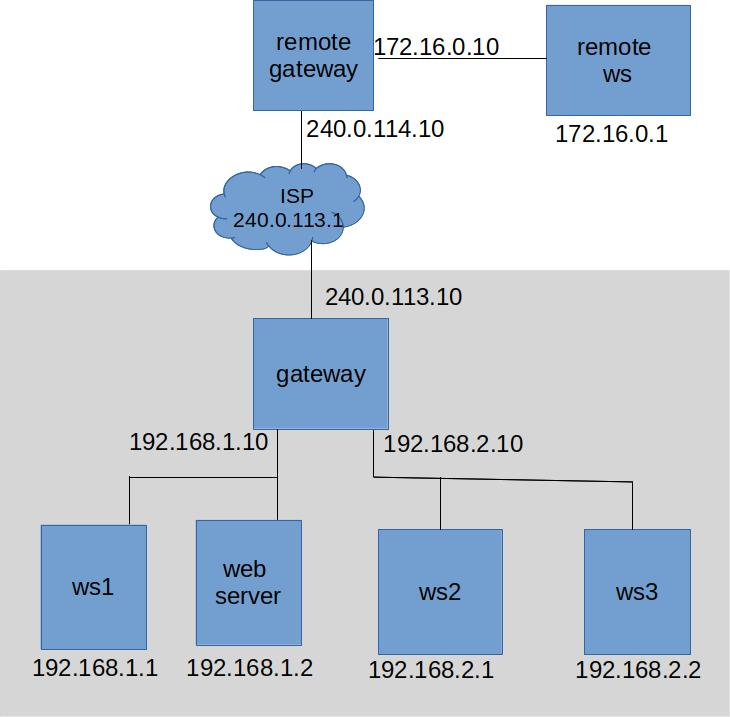
\includegraphics [width=0.8\textwidth]{routing-basics.jpg}
\end{center}
\caption{Network topology for routing-basics lab}
\label{fig:topology}
\end{figure}

This lab is designed to avoid use of name servers for the local computers, the intention is to focus
on IP addresses and network interfaces.

\section{Lab Tasks}
\subsection{Explore}
Use {\tt ifconfig} or {\tt ip addr} on the different computers to familiarize yourself with
the subnets associated with each of the computer's network interfaces.
Note how ws2 and ws3 are on the same subnet, yet ws1 and the web server are on a different subnet.
And note how the gatway has a network interface on the same subnet as ws1, and a different
network interface on the same subnet as ws2 and ws3.

\subsection{Internal Packet Forwarding}
From each of the three workstations, enter the following command:
\begin{verbatim}
    route -n
\end{verbatim}
\noindent Note how ws1 and ws2 include routing table entries that name the
gateway as the \textit{default gateway}.  For example, on ws1 the routing table can be read as:
``If the destination address is on my eth0 subnet, (192.168.1.0/24), use the eth0 interface
and ARP to locate the destination.  Otherwise, send the packet to the gateway (192.168.1.10).'' 
This allows ws1 and ws2 to address each other, which 
can be demonstrated by using \texttt{ping} from ws1 to reach ws2 via the gateway.  First start
{\tt tcpdump} on the gateway to view traffic on the two network interfaces\footnote{use the -n option to prevent tcpdump from
using reverse DNS to put names to IP address and ports.}:   
\begin{verbatim}
   sudo tcpdump -i eth0 -n -vv
\end{verbatim}

\noindent Then, on ws1:
\begin{verbatim}
    ping [ws2 IP] -c 3
\end{verbatim}

Now consider ws2 and ws3.  Since they are both on the same subnet, they can ping
each other.  Try that for yourself. And look at the tcpdump output on your gateway
and note how the only new activity is an ARP request from whichever workstation you
issued the ping from. 

Next, try to ping ws1 from ws3.  That fails because ws3 has no routing table entry defining what to do with traffic 
that is not destined for a subnetwork of one of the ws3 interfaces.

On ws3, define the gateway component as the \textit{default gateway} using the 
\texttt{route} command, but this time using \texttt{sudo} because we are altering the routing:

\begin{verbatim}
    sudo route add default gw [gateway IP]
\end{verbatim}
\noindent Then try to ping ws1 from ws3.  The ws3 routing table now knows what
to do with packet addressed to ws1.  You should now also be able to reach the web server
from ws3, try that:
\begin{verbatim}
    wget 192.168.1.2
\end{verbatim}  
This is a temporary routing table fix that will revert if the
system is restarted, but it can be made permenant with techniques not covered here.

\subsection{Routing to the Internet}
The gateway component is configured to forward packets to a simulated ISP at 203.0.113.1, which 
is a hidden component that provides routing to the Internet for this lab.  From ws2, 
try to {\tt wget www.google.com}.  Then do the same from ws3.  The problem with ws3 is that
it has no domain name service (DNS) definition.  Note, routing from ws3 to the Internet
works fine, which you can confirm by pinging the IP address of www.google.com (as displayed
when you pinged from ws2).  The ws3 component simply lacks a DNS definition. 
On ws2, the DNS is defined to be the
gateway component, and this is achieved in the \texttt{/etc/resolv.conf} file \footnote{
Many Linux systems include functions for defining your DNS, and these tools will overwrite
the resolv.conf file.  So modifying the {\tt resolv.conf} file may be only a temporary
fix, which is sufficient for this lab.}.  If you 
modify the {\tt resolv.conf} file on ws3 to match that of ws2, that will tell ws3 to use the gateway
as its DNS.  (While the gateway is not a DNS, it runs a \textit{dnsmasq} service to forward DNS requests to
the DNS that it uses.)   Modify the {\tt resolv.conf} file and confirm you can resolve the www.google.com
address using {\tt wget www.google.com}.  Use {\tt sudo vi} or {\tt sudo nano} to modify the file.  See the 
{\tt nix-commands} lab if you are not familiar with text editors.

\subsection{Use of Network Address Translation (NAT)}
Now, review how the gateway component implements NAT using the \texttt{iptables} 
utility.  Consider traffic from ws1 destined for www.google.com. The source IP address
on those packets is 192.168.1.1.  The ws1 component sends the packets to its default
gateway, i.e., our gateway component.  The gateway routing table is configured to
send external traffic to the simulated ISP at 203.0.113.1.  However, before that traffic is sent, we need
to translate the source IP address to our exernal 203.0.113.10 address so that google or our ISP knows
where to send replies.  
Use this command on the gatway (use ctrl-c to break out of tcpdump if it is running):
\begin{verbatim}
    sudo iptables -L -v -t nat
\end{verbatim}
\noindent to view our single NAT rule, having a target of \texttt{MASQUERADE}, which will translate
source addresses for all traffic destined for our external network interface. (The other 2 NAT rules will
be discussed in the following section.) 

These iptables rules are defined in the /etc/rc.local file on the gateway component.  

Use {\tt wget google.com} from ws1 and observe the source IP address in the tcpdump on the gateway's interface
to the subnet containing ws1.  Then use ctrl-c to stop tcpdump and restart it on the gateway's
network interface on the ISP's subnet:
\begin{verbatim}
   sudo tcpdump -i eth2 -vv -n
\end{verbatim}
\noindent And then wget again.  Note how the source address of the packets has changed.

This illustrates the use of NAT to share a single IP address amongst many computers.  Here,
the enterprise has but a single externally addressable IP address, yet all of the workstations are able to 
access services on the Internet.

\subsection{Services behind NAT}
Another property of NAT is that it ``hides'' local computers from the internet, thereby providing some
ad-hoc security.  Go to the remote workstation
({\tt remote\_ws}) and try to ping ws1.  External to our gateway, there is no way to name the ws1 computer other than
via the mapping within the gateway that allows it to forward traffic destined ws1 for sessions \textit{initiated} by ws1.
As a result of NAT, nothing on the internet can initiate a connection with the internal workstations.  

There are situations in which you want external systems to be able to initiate connections to services that would
otherwise be hidden by NAT.
NAT rules can be configured to map port numbers of incoming traffic to internal components.  For example, the gateway
is configured to route web requests on port 80 to the web server.  Revisit the output of the
\begin{verbatim}
    sudo iptables -L -v -n -t nat
\end{verbatim}
command. You will notice a \textit{Destination NAT} (DNAT) rule in the PREROUTING chain and 
a \textit{Source NAT} (SNAT) rule in the POSTROUTING chain. 
The DNAT rule directs the iptables to replace the destination address with the address of the web server before
deciding how to route the packet.
The SNAT rule directs iptables to replace the source address with the gateway's address prior to sending
the packet to the web server (i.e., after deciding how to route the packet).

Restart your tcpdump on eth0 on the gateway.   Then query the web server from the remote workstation:
\begin{verbatim}
    wget 203.0.113.10
\end{verbatim}
Observe how the destination address is the web server, and the source address is the gateway.

Note the security implications of these SNAT and DNAT rules.  The web server is now accessible to the 
entire Internet, and this increases the risks to the other computers since they can be addressed
by the web server. If the web server becomes compromised, it can be used to attack internal computers.
See the {\tt dmz-lab} for an exercise illustrating potential solutions to that problem. 

\section{Submission}
After finishing the lab, go to the terminal on your Linux system that was used to start the lab and type:
\begin{verbatim}
    stoplab 
\end{verbatim}
When you stop the lab, the system will display a path to the zipped lab results on your Linux system.  Provide that file to 
your instructor, e.g., via the Sakai site.

\copyrightnotice

\end{document}
